% !TEX program = xelatex

\documentclass[12pt]{article}
\usepackage{ctex}
\usepackage{amsmath}
\usepackage{geometry}
\usepackage{graphicx}
\usepackage{float}
\usepackage{hyperref}

\geometry{a4paper, margin=2.5cm}

\title{计算机图形学作业一：MiniDraw 实验报告}
\author{姓名：胡广理 \quad 学号： PB24010500}
\date{\today}

\begin{document}
\maketitle

\section{实验目的}
本实验旨在通过 C++ 编程与 ImGui 框架，实现一个简单的二维矢量绘图软件（MiniDraw）。要求掌握面向对象的图形系统设计方法，实现常用的几何图元（如直线、矩形、椭圆、多边形等）的绘制与交互，理解并实践图形学中基础的交互逻辑（鼠标事件处理）以及动态重绘机制。

\section{实验环境}
\begin{itemize}
    \item 操作系统：Linux
    \item 编程语言：C++ (C++17)
    \item 编译构建系统：CMake
    \item 图形库/GUI框架：OpenGL, GLFW, ImGui
\end{itemize}

\section{系统架构与类图设计}
由于系统中可能包含多种类型的图元实体，实验采用了多态的方式对图元进行管理。所有具体图元（如 \texttt{Line}, \texttt{Rect}, \texttt{Ellipse}, \texttt{Polygon} 等）均继承自一个公共基类 \texttt{Shape}。基类中定义了绘制 \texttt{draw()} 以及用于交互状态更新的虚函数，子类各自覆盖这些方法实现不同的绘制行为。

画布区域继承自系统的图形控件 \texttt{CanvasWidget}，画布负责维护一个存放 \texttt{Shape} 指针的列表，捕捉用户的鼠标点击、拖拽信号，并下发给当前处于活动状态的图元进行构造或是选择。

下图展示了 MiniDraw 系统的核心类图架构：

\begin{figure}[H]
    \centering
    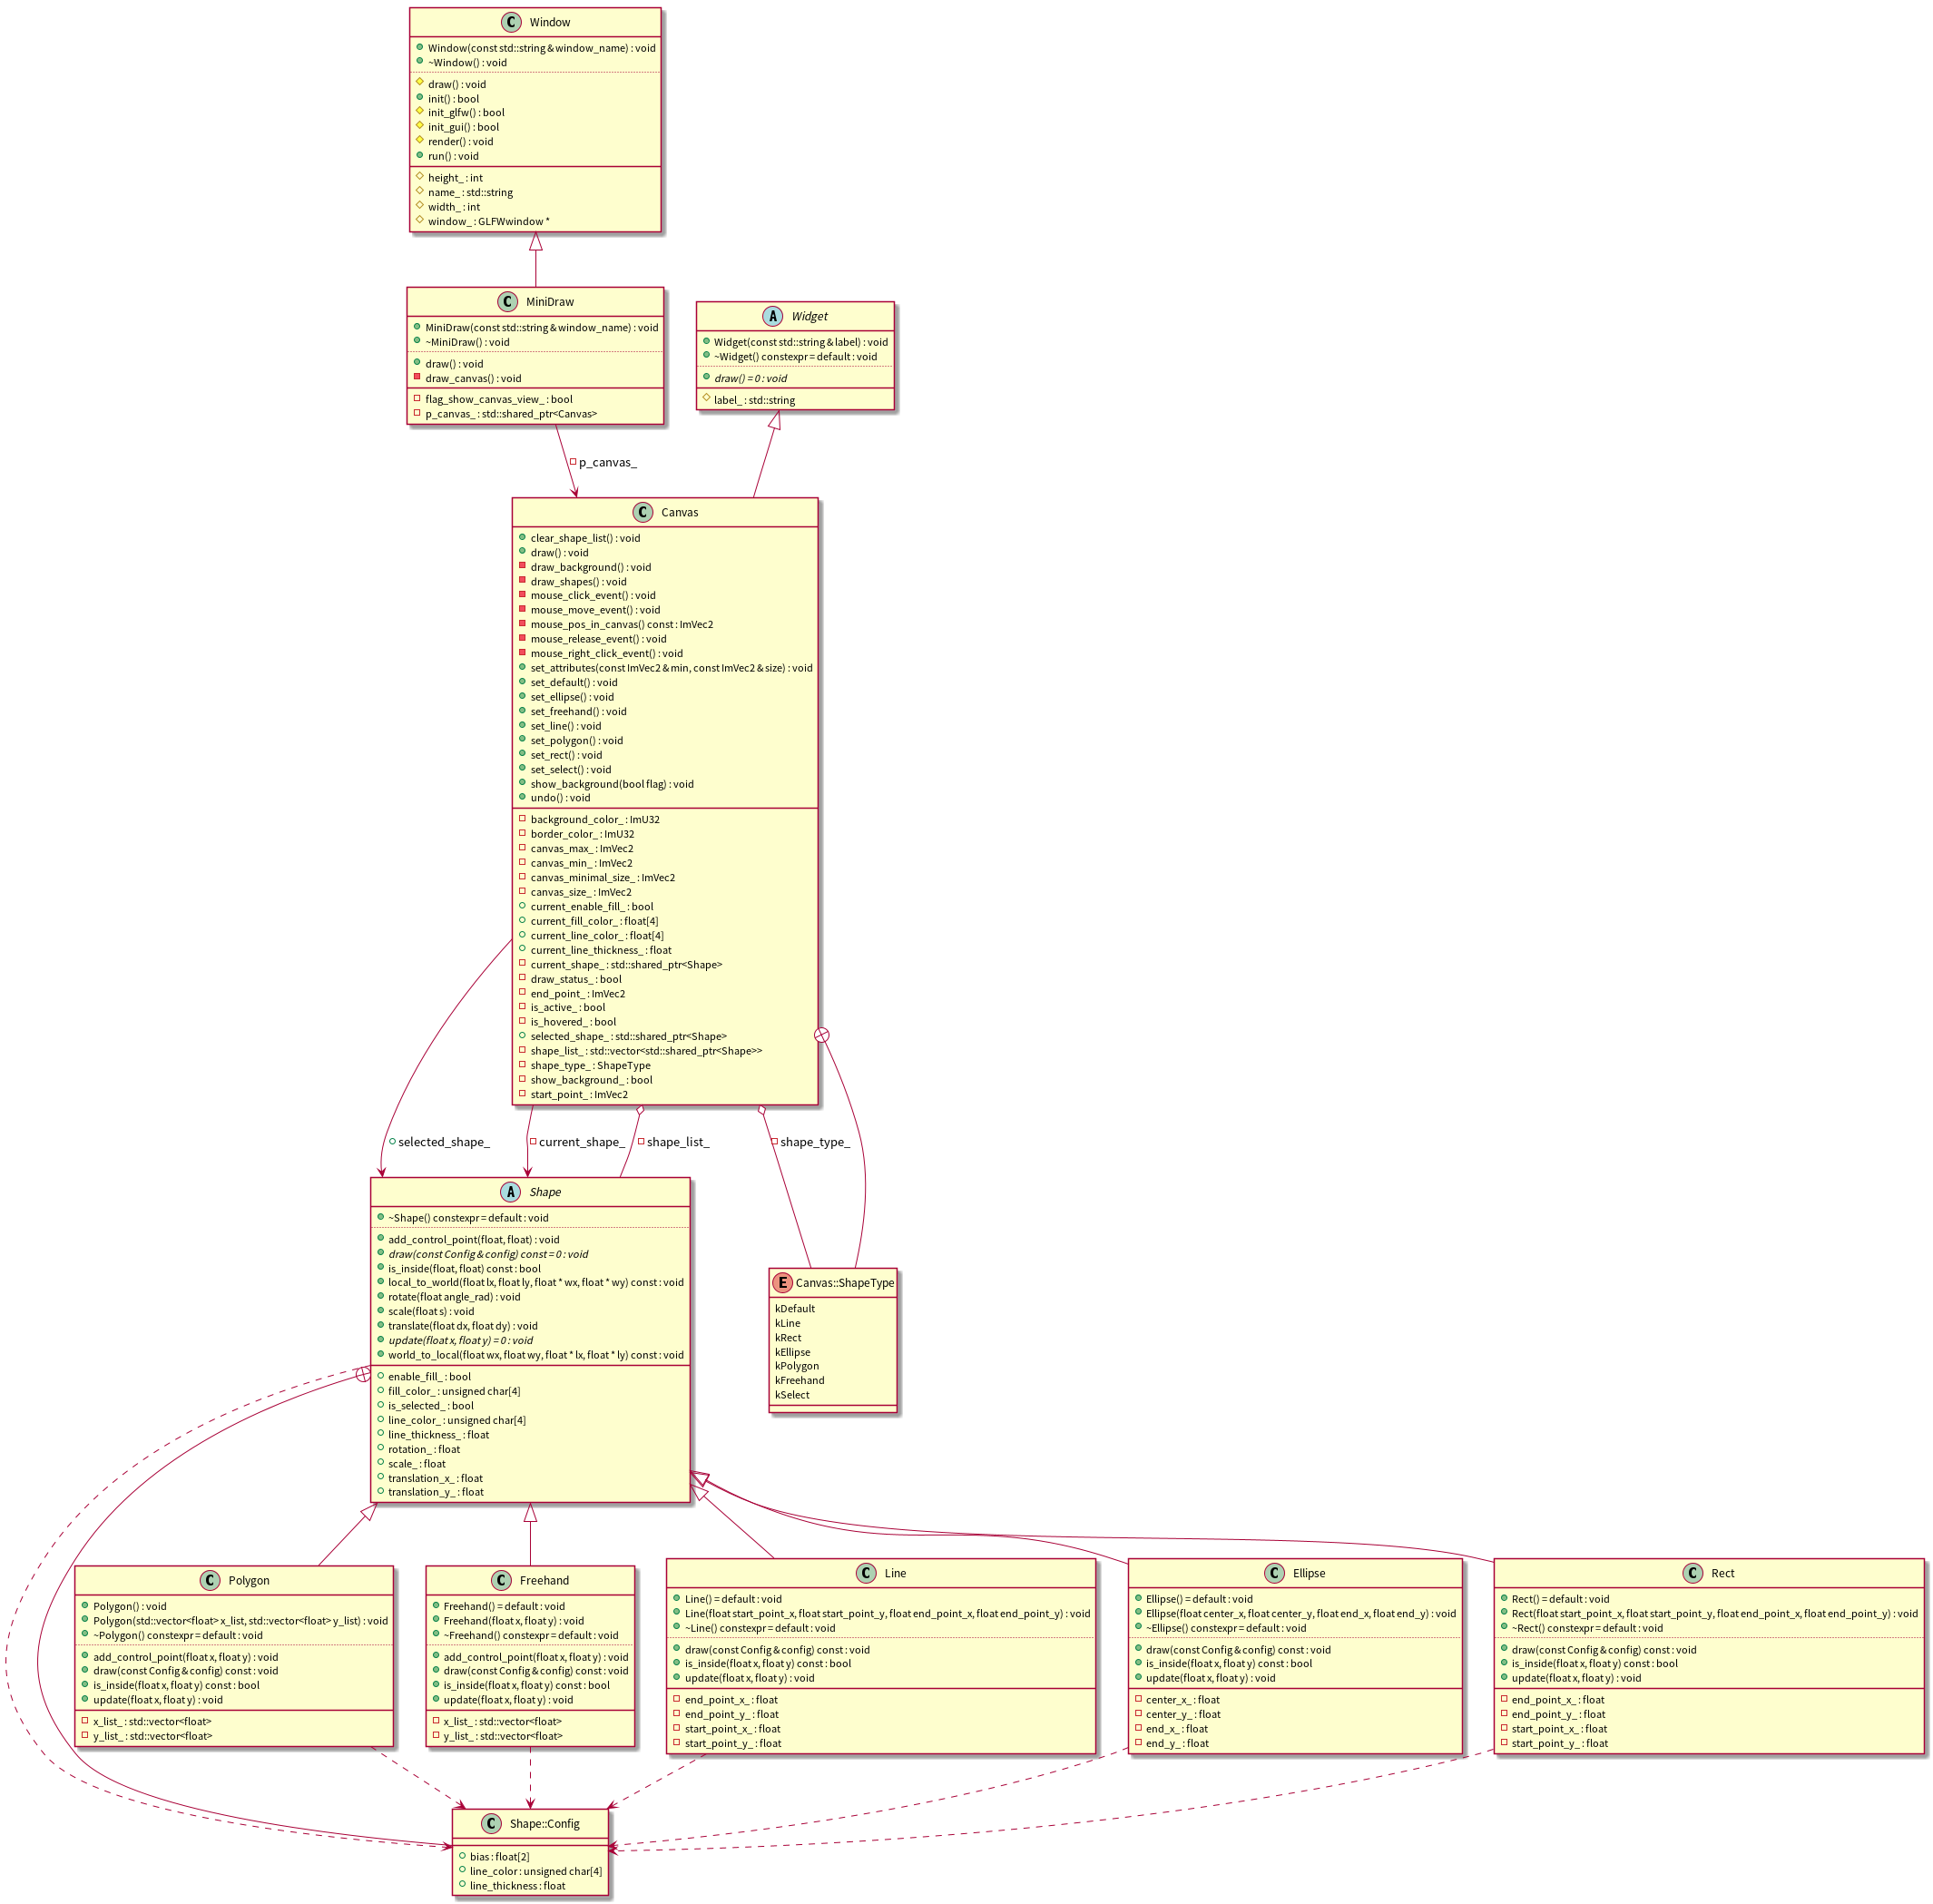
\includegraphics[width=0.8\textwidth]{diagrams/1_MiniDraw.png}
    \caption{MiniDraw 类图结构（面向对象设计）}
    \label{fig:class_diagram}
\end{figure}

\section{核心功能实现与交互逻辑}

\subsection{图元类的定义}
基类 \texttt{Shape} 存储了图元颜色、粗细等通用属性，子类各自保留描述自身几何形状所需的控制点（如线段的起点与终点、多边形的顶点数组等）。
在重写 \texttt{draw()} 接口时，调用 ImGui 提供的底层绘制 API（如 \texttt{ImDrawList::AddLine}, \texttt{ImDrawList::AddRect} 等）在画布上输出几何图形。

\subsection{用户交互与状态机管理}
在 \texttt{CanvasWidget} 的更新循环中，系统不断检测用户的鼠标状态：
\begin{enumerate}
    \item \textbf{鼠标按下 (MouseDown)：} 若在绘制模式下，根据当前选定的图元类型工厂（Factory）实例化对应图元对象，并保存初始控制点；
    \item \textbf{鼠标拖拽 (MouseDrag)：} 更新当前正在绘制的图元的动态控制点（例如矩形的对角点），实现“所见即所得”的橡皮筋拉伸反馈；
    \item \textbf{鼠标释放 (MouseRelease)：} 确认并固化当前图元，终止绘制状态机。
\end{enumerate}
对于多边形绘制等更复杂的操作，系统根据左右键的不同分别处理点集的添加与闭合状态。

\section{实验结果与展示}
在完成各项图元的交互逻辑和界面功能后，运行程序可以正常进行画图操作。通过控制面板，用户可以切换画笔颜色、粗细，并选择不同的绘制工具。画布中央能够正确响应鼠标的各项操作，实时预览画面的结果并且支持叠加绘制。

以下是使用本程序的综合绘制最终效果图：

\begin{figure}[H]
    \centering
    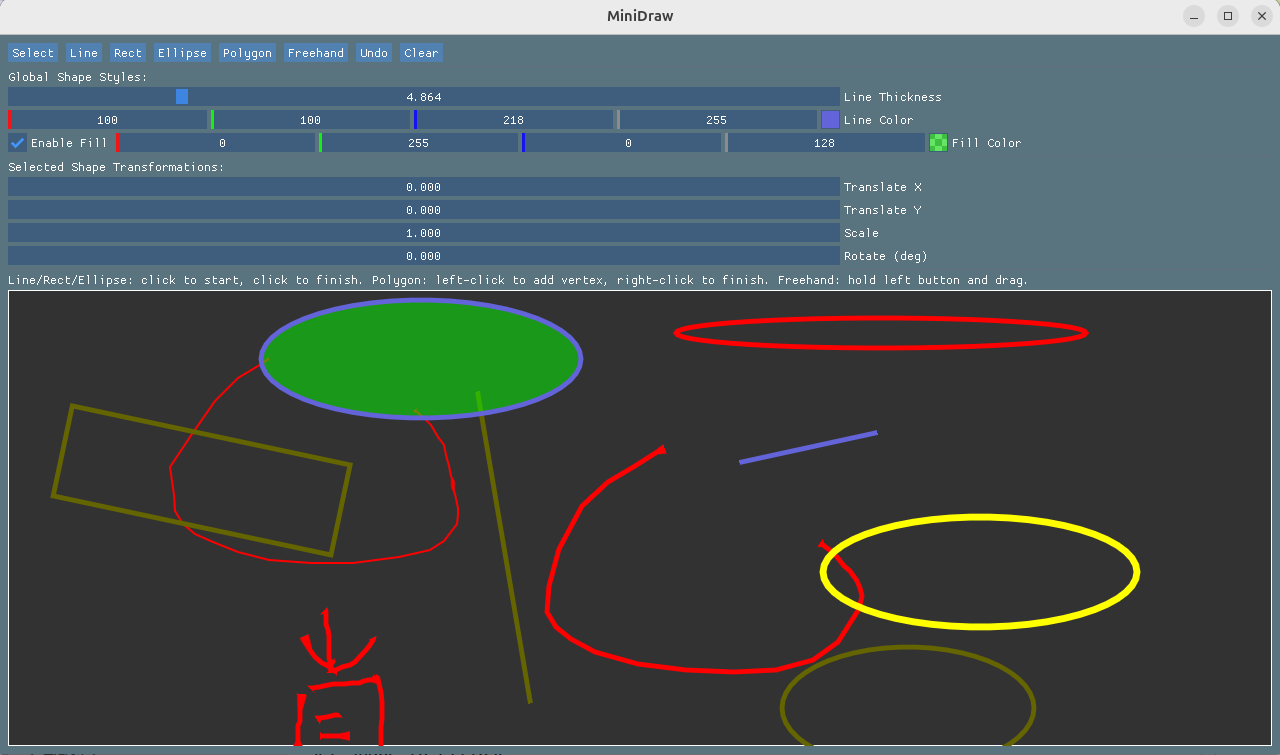
\includegraphics[width=0.9\textwidth]{diagrams/效果图.png}
    \caption{MiniDraw 实验运行效果图}
    \label{fig:result}
\end{figure}

\section{实验总结}
通过本次 MiniDraw 实验，我深刻理解了矢量图形软件底层的数据维护和交互事件分发原理。通过运用继承与多态，降低了系统的耦合度，方便以后轻松接入更多类型的曲线与图形单元。同时，利用 ImGui 作为前端界面极大地简化了窗口与图形上下文管理部分的代码，帮助我将核心精力聚焦在图形逻辑的开发上。实验过程不仅提升了我的 C++ 面向对象编程能力，也为后续复杂图形学算法的实现搭建了坚实的基础框架。

\end{document}

